\documentclass[tikz]{standalone}
\usepackage{tikz}
\usepackage{standalone}
\begin{document}	
	
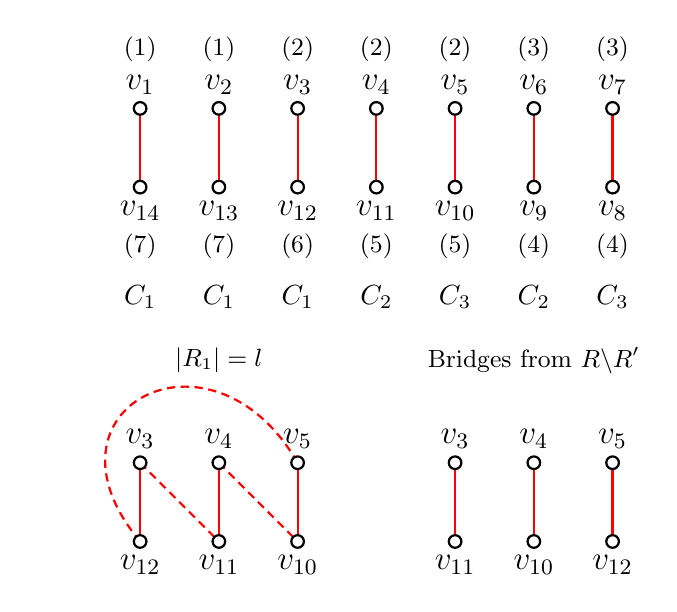
\begin{tikzpicture}
%\draw [help lines] (-1,-1) grid (9, 10);

% LIST OF EDGES FOR MBR.
\draw [thick, red] (1,7.5) -- (1,8.5);
\draw [thick, red] (2,7.5) -- (2,8.5);
\draw [thick, red] (3,7.5) -- (3,8.5);
\draw [thick, red] (4,7.5) -- (4,8.5);
\draw [thick, red] (5,7.5) -- (5,8.5);
\draw [thick, red] (6,7.5) -- (6,8.5);
\draw [thick, red] (7,7.5) -- (7,8.5);

\draw [fill=white, thick] (1,7.5) circle [radius = 0.08];
\draw [fill=white, thick] (2,7.5) circle [radius = 0.08];
\draw [fill=white, thick] (3,7.5) circle [radius = 0.08];
\draw [fill=white, thick] (4,7.5) circle [radius = 0.08];
\draw [fill=white, thick] (5,7.5) circle [radius = 0.08];
\draw [fill=white, thick] (6,7.5) circle [radius = 0.08];
\draw [fill=white, thick] (7,7.5) circle [radius = 0.08];
\draw [fill=white, thick] (1,8.5) circle [radius = 0.08];
\draw [fill=white, thick] (2,8.5) circle [radius = 0.08];
\draw [fill=white, thick] (3,8.5) circle [radius = 0.08];
\draw [fill=white, thick] (4,8.5) circle [radius = 0.08];
\draw [fill=white, thick] (5,8.5) circle [radius = 0.08];
\draw [fill=white, thick] (6,8.5) circle [radius = 0.08];
\draw [fill=white, thick] (7,8.5) circle [radius = 0.08];

\node at (1,7.2) {\large{$v_{14}$}};
\node at (2,7.2) {\large{$v_{13}$}};
\node at (3,7.2) {\large{$v_{12}$}};
\node at (4,7.2) {\large{$v_{11}$}};
\node at (5,7.2) {\large{$v_{10}$}};
\node at (6,7.2) {\large{$v_9$}};
\node at (7,7.2) {\large{$v_8$}};

\node at (1,8.8) {\large{$v_1$}};
\node at (2,8.8) {\large{$v_2$}};
\node at (3,8.8) {\large{$v_3$}};
\node at (4,8.8) {\large{$v_4$}};
\node at (5,8.8) {\large{$v_5$}};
\node at (6,8.8) {\large{$v_6$}};
\node at (7,8.8) {\large{$v_7$}};

\node at (1,6.75) {\small{(7)}};
\node at (2,6.75) {\small{(7)}};
\node at (3,6.75) {\small{(6)}};
\node at (4,6.75) {\small{(5)}};
\node at (5,6.75) {\small{(5)}};
\node at (6,6.75) {\small{(4)}};
\node at (7,6.75) {\small{(4)}};

\node at (1,9.25) {\small{(1)}};
\node at (2,9.25) {\small{(1)}};
\node at (3,9.25) {\small{(2)}};
\node at (4,9.25) {\small{(2)}};
\node at (5,9.25) {\small{(2)}};
\node at (6,9.25) {\small{(3)}};
\node at (7,9.25) {\small{(3)}};

\node at (1,6.1) {$C_1$};
\node at (2,6.1) {$C_1$};
\node at (3,6.1) {$C_1$};
\node at (4,6.1) {$C_2$};
\node at (5,6.1) {$C_3$};
\node at (6,6.1) {$C_2$};
\node at (7,6.1) {$C_3$};

%\node at (4,5.15) {$R_1 = \{(v_3, v_{12}), (v_4, v_{11}), (v_5, v_{10})\}$};

%----------------------------------------------------------------
% EDGES IN SET R1 WITH EDGES FROM R\R' DASHED, CONNECTING PROCEDURE.
\node at (2,5.3) {\small{$|R_1| = l$}};

\draw [thick, red] (1,3) -- (1,4);
\draw [thick, red] (2,3) -- (2,4);
\draw [thick, red] (3,3) -- (3,4);

\draw [thick, densely dashed, red] (1,4) -- (2,3);
\draw [thick, densely dashed, red] (2,4) -- (3,3);
\draw [thick, densely dashed, red] (3,4) to[out=120,in=130, distance=2.2cm] (1,3);

\draw [fill=white, thick] (1,3) circle [radius = 0.08];
\draw [fill=white, thick] (2,3) circle [radius = 0.08];
\draw [fill=white, thick] (3,3) circle [radius = 0.08];
\draw [fill=white, thick] (1,4) circle [radius = 0.08];
\draw [fill=white, thick] (2,4) circle [radius = 0.08];
\draw [fill=white, thick] (3,4) circle [radius = 0.08];

\node at (1,2.7) {\large{$v_{12}$}};
\node at (2,2.7) {\large{$v_{11}$}};
\node at (3,2.7) {\large{$v_{10}$}};
\node at (1,4.3) {\large{$v_3$}};
\node at (2,4.3) {\large{$v_4$}};
\node at (3,4.3) {\large{$v_5$}};

%-------------------------------------------
% EDGES FROM R\R' FOUND USING MBR AND CONNECTING PROCEDURE, USE TO CONNECT CYCLES.
\node at (6,5.3) {\small{Bridges from $R\backslash R'$}};

\draw [thick, red] (5,3) -- (5,4);
\draw [thick, red] (6,3) -- (6,4);
\draw [thick, red] (7,3) -- (7,4);

\draw [fill=white, thick] (5,3) circle [radius = 0.08];
\draw [fill=white, thick] (6,3) circle [radius = 0.08];
\draw [fill=white, thick] (7,3) circle [radius = 0.08];
\draw [fill=white, thick] (5,4) circle [radius = 0.08];
\draw [fill=white, thick] (6,4) circle [radius = 0.08];
\draw [fill=white, thick] (7,4) circle [radius = 0.08];

\node at (5,2.7) {\large{$v_{11}$}};
\node at (6,2.7) {\large{$v_{10}$}};
\node at (7,2.7) {\large{$v_{12}$}};
\node at (5,4.3) {\large{$v_3$}};
\node at (6,4.3) {\large{$v_4$}};
\node at (7,4.3) {\large{$v_5$}};

\end{tikzpicture}
	
\end{document}